\documentclass[11pt]{scrartcl}
\usepackage{dominatrix}
\usepackage{colortbl}
\usepackage{pgfplots}
\newcommand{\jon}{Jón }
\pgfplotsset{compat=1.9}
\renewcommand\thesubsection{\alph{subsection}}
\definecolor{light-gray}{gray}{0.75}
\title{Mathematics Crash Course}
\subject{ECON W3213 Spring 2014 \jon Steinsson}
\author{Linan Qiu, lq2137}
\begin{document}
\maketitle

\begin{abstract}
This set of recitation notes covers \textbf{Partial Derivatives}, \textbf{Taylor Series Approximation}, and \textbf{Optimization}. More content may be added as more mathematical techniques are employed during the course of this lesson. This is \textbf{not} a substitute for a proper mathematics education. That being said, we do want to apply all that intellectual shebang to something more than 2D curves and 3D planes right? Attaboy.
\end{abstract}

\section{Partial Derivatives}

\subsection{How to Partial Differentiate}
Forget the intimidating name. Partial derivatives is really nothing too different from what you've known to be \textbf{differentiation} all along.

Let's say we're interested in the GPA that you get at the end of this course. We all agree that the more sessions of Linan's recitations you attend, the higher a GPA you get. You have to agree with that. That is the truth.

With $G$ being the \textbf{GPA} you get, and $r$ being the number of \textbf{recitations} you attend, we can create a function like this

\[G(r) = \log{r} + 1 \]

If I ask you, "if you attend one more of Linan's recitations, how much higher will your GPA be?" You'd probably answer, "Let me differentiate this with respect to $r$!" So we have

\[ \frac{d G(r)}{d r} = \frac{1}{r} \]

The derivation of the equation above is left as an exercise to the reader. 

Now say we're even more interested in your GPA. We'll then consider the amount of \textbf{vodka} $v$ that you drink. In that case, we can write

\[G(r, v) = \log{r} - v + 1\] 

$G(r,v)$ means that $G$ as a function depends on both $r$, recitations, and $v$, vodka. Of course vodka makes you dumber. 

Now say we still want to investigate the effect of attending one more of Linan's recitations. 

But this time, we have a variable $v$ to deal with! Then we have to \emph{hold the amount of vodka constant}. Why? If we don't do that, then we won't know if the effect on GPA is contributed by $r$ or $v$. So in that case, we treat $v$ as a constant.

If we treat $v$ as a constant, this means

\[\frac{\partial G(r,v)}{\partial r} = \frac{1}{r} - 0 + 0 = \frac{1}{r}\]

Let's see why this happens. In treating $v$ as a constant, we are saying that $\frac{d v}{d r} = 0$, as is any other variable (for example in the constant 1, $\frac{d 1}{d r} = 0$).

This effectively means 

\begin{quote}
Holding the amount of vodka I drink constant, if I attend one more of Linan's recitations, my GPA will increase by $\frac{1}{r}$
\end{quote}

Note that I used $\partial$ instead of the conventional $d$ for $\frac{\partial G(r,v)}{\partial r}$ to denote that I'm only differentiating $G(r,v)$ with respect to one of its variables $r$, and not the other variable $v$. That's why we call this \textbf{partial} differentiation!

We can do this for vodka too!

\[\frac{\partial G(r,v)}{\partial v} = 0 - 1 + 0 = -1 \]

In this case, we treat $r$ as a constant. Then $\log{r}$ is a constant as well, which then results in it becoming $0$ when differentiation with respect to $v$. 

This effectively means

\begin{quote}
Holding the recitations I go to constant, if I drink one more liter of vodka, my GPA goes down by $1$.
\end{quote}

Fair assumption eh?

Now let me try screwing around with you a little. Let's say I want to include so darn many factors, like 

\begin{itemize}
	\item $f$, the amount of time you spend on Facebook a day
	\item $s$, the number of hours you sleep a night
	\item $c$, the level of calculus class that you've taken
	\item $g$, the amount of games you play on the computer
\end{itemize}

We end up with a monster like this

\[ G(r,v,f,s,c,g) = \log{r}s^f + e^{s} - vs^2 - c^g - \frac{f}{scg \frac{v^2}{\log{f}}}+ 1 \]

Let's find the partial derivative of $G$ with respect to $r$ again. This is one heck of a monster, but that we keep all other variables constant. 

Hence, this simply evaluates to

\[ \frac{\partial G(r,v,f,s,c,g)}{\partial r} = \frac{s^f}{r} \]

The rest of it simply vanished since we treat it as a constant. Get the hang of it?

Let's try applying this to economics. 

\subsection{Application in Economics}
\jon used this animal for the production function

\[ Y(K,L) = \bar{A}K^{\alpha}L^{1 - \alpha} \]

(Note that the bar above $\bar{A}$ simply means that it remains constant and isn't a variable.)

Now if we want to find the effect of changing $K$ on $Y$, we have to hold $L$ constant. We'd treat $L$ as a constant. In that case,

\[ \frac{\partial Y(K,L)}{\partial K} = \bar{A} L^{1 - \alpha} (\alpha K^{\alpha-1}) \]

What has happened? We treated $L$ as a constant, so $L^{1-\alpha}$ is a constant. So we simply treat is as any other coefficient during differentiation. Then, the animal in the bracket on the RHS is simply the result of differentiating $K^{\alpha}$ with respect to $K$, which yields us $\alpha K^{\alpha - 1}$

This effectively means

\begin{quote}
Holding the amount of labor constant, if I increase capital $K$ by one unit, production $Y$ will increase by $\bar{A} L^{1 - \alpha} (\alpha K^{\alpha-1})$ units.
\end{quote}

Let's do the same for $L$. 

\[ \frac{\partial Y(K,L)}{\partial L} = \bar{A}K^{\alpha}((1-\alpha)L^{-\alpha}) \] 

Again, we treat $K$ as a constant this time. Differentiating $L^{1-\alpha}$ with respect to $L$ gives us $(1-\alpha)L^{-\alpha})$

\section{Optimization}

\subsection{How to Optimize}

Optimization comes in two types:

\begin{enumerate}
	\item Unconstrained
	\item Constrained
\end{enumerate}

\subsubsection{Unconstrained Optimization}
\begin{figure}[ht!]
\centering
\begin{tikzpicture}
\begin{axis}[]
\addplot[domain=-3:2,black]
{(x^2)};
\addplot[domain=-3:2,black, dotted]
{0};
\end{axis}
\end{tikzpicture}
\caption{Plot of $y = x^2$}
\end{figure}

The plot above is of $y = x^2$. If I ask you to find the minima of the function, you'll say that it is at $x=0$. Obviously it is. If I ask you to find the maxima of the function, you'll say that there is no maxima, since it tends towards positive infinity.

When we do unconstrained optimization, we are simply trying to find the \textbf{maxima} and \textbf{minina} \emph{without any constraints}. 

\subsubsection{Constrained Optimization}

Now what do \textbf{constraints} mean?

\begin{figure}[ht!]
\centering
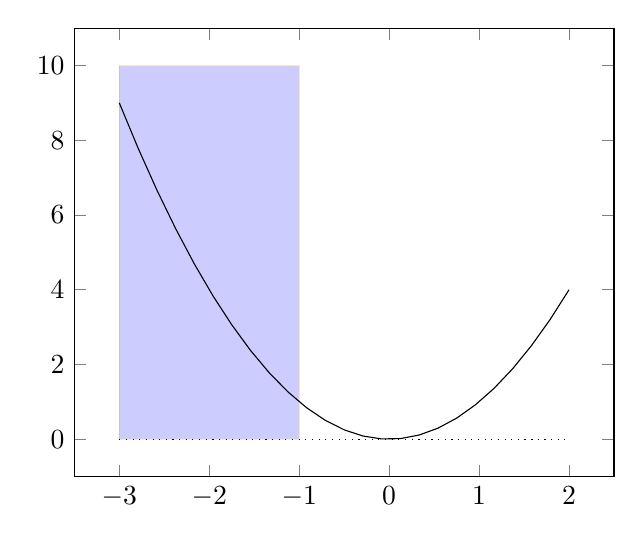
\begin{tikzpicture}
\begin{axis}[]
\addplot[patch,patch type=rectangle,blue,opacity=0.2]
coordinates {(-3,10) (-3, 0) (-1, 0) (-1, 10)};
\addplot[domain=-3:2,black]
{(x^2)};
\addplot[domain=-3:2,black, dotted]
{0};
\end{axis}
\end{tikzpicture}
\caption{Plot of $y = x^2$}
\end{figure}

If I limit the plot to be between the domain of $-3 \leq x \leq -1$, then what is the maxima and minima? The minima is no longer $y=0$, since $x=0$ lies beyond the domain allowed for by my constraint. Then in that case, the minima will be $y = (-1)^2 = 1$ and the maxima will be $y = (-3)^2 = 9$.

\begin{figure}[H]
\centering
\begin{tikzpicture}
\begin{axis}[]
\addplot[domain=-3:2,black]
{(x-1)*(x+1)*(x+2)};
\addplot[domain=-3:2,black, dotted]
{0.631};
\addplot[domain=-3:2,black, dotted]
{-2.1125};
\end{axis}
\end{tikzpicture}
\caption{Plot of $y = (x-1)*(x+1)*(x+2)$}
\end{figure}

When given a function like this, you should understand by now that we won't be able to yield a maxima or minima unless we limit the function to a certain range. This is why constrained optimization can be useful sometimes -- it yields us meaningful results. That curve, for example, could be the output for a factory given differing amounts of input. We won't be interested in what the output will be if input was infinity. Instead, we'd want to set a limit for inputs and find the maximum output we can produce.

In short, 

\begin{enumerate}
	\item Unconstrained: maximize / minimize one single function
	\item Constrained: maximize / minimize the function subject to a certain \textbf{limitation}, or what we call the constraint. There are several ways we can deal with constrained optimization
	\begin{itemize}
		\item Plug and substitute (this is the method we are using)
		\item Lagrangian (you will learn this in Calc III. No need to use it in this course.)
	\end{itemize}
\end{enumerate}

Let's see how \jon used this in macroeconomics.

\subsection{Application to Economics}

\subsubsection{Unconstrained Optimization}

Consider the profit maximization problem

\[ \max \Pi =AK^{\alpha }L^{\beta }-wL-rK \]

where $\alpha ,\beta <1$

Remember \textbf{partial differentiation}? Let's use it!

\begin{align*}
\frac{\partial \Pi }{\partial K} &= A\alpha K^{\alpha -1}L^{\beta }-r=0 \\
\frac{\partial \Pi }{\partial L} &= A\beta K^{\alpha }L^{\beta -1}-w=0
\end{align*}

From this, we know that

\begin{align*}
r &= A\alpha K^{\alpha -1}L^{\beta } \\
w &= A\beta K^{\alpha }L^{\beta -1}
\end{align*}

We used these two equations to gain insights on the behavior of firms. We did so by optimizing (maximizing) the profit that the firm gets. Did we subject the firm's $K$ and $L$ to any constraints? Nope! Hence this is an example of unconstrained optimization.

Can we add conditions to this? Of course. For example, we can make up a condition like $L = K$ In that case, we simply substitute this condition $L=K$ into our solutions to solve for $r$ and $w$ in terms of $K$ or $L$. However, this \textbf{does not make economic sense}. Instead, let's look at something that does.

\subsubsection{Cosntrained Optimization}

Now consider this household problem

\begin{align*}
\max U\left( c,H\right)  &= a\ln c+b\ln \left( 1-H\right)  \\
st : pc &= wH
\end{align*}

Our first step is to substitute the constraint into the problem

\begin{align*}
\max a\ln c+b\ln \left( 1-H\right) \\
=a\ln \left[ \frac{wH}{p}\right] +b\ln (1-H)
\end{align*}

Now all we have to do is to solve it like the \textbf{unconstrained optimization}. Differentiate with respect to $H$

\begin{align*}
\frac{awp}{wHp} =\frac{b}{1-H} &\implies \frac{\frac{b}{1-H}}{\frac{a}{c}}=\frac{w}{p} \\
&\implies H^*=\frac{a}{a+b} \\
& \implies c^{\ast }=\frac{wa}{a+b}
\end{align*}

We now make sense of this by saying that the condition that 

\[ \frac{\frac{b}{1-H}}{\frac{a}{c}}=\frac{w}{p}\]means the marginal rate of substitution between working and consumption is the wage.

\section{Taylor Series Expansion}

\subsection{What is Taylor Series?}

Taylor Series Expansion is the idea that a smooth function can be approximated by a polynomial. Think of it as curve fitting.

Imagine you have a function $f(x)$.

\begin{figure}[ht!]
\centering
\begin{tikzpicture}
\begin{axis}[]
\addplot[domain=-2:2,black]
{e^x};
\addplot[mark=*, blue, mark size=3pt]
coordinates {(1,e)};
\end{axis}
\end{tikzpicture}
\caption{Plot of $f(x)$}
\end{figure}

We can pick a point $(1, e)$ marked above. We can also find the tangent of the curve at that point.

\begin{figure}[ht!]
\centering
\begin{tikzpicture}
\begin{axis}[]
\addplot[domain=-2:2,black]
{e^x};
\addplot[mark=*, blue, mark size=3pt]
coordinates {(1,e)};
\addplot[domain=0:2,blue]
{e*x};
\end{axis}
\end{tikzpicture}
\caption{Plot of $f(x)$ with tangent at $(1, e)$}
\end{figure}

Around $x = 1$, the tangent is a \emph{pretty} good approximation of the original $f(x)$. However, if we move large distances away from $x=1$, say at $x=3$ or $x=-2$, then the value indicated by $f(3)$ or $f(-2)$ will be very different from the value given by the tangent line. 

\begin{figure}[ht!]
\centering
\begin{tikzpicture}
\begin{axis}[]
\addplot[domain=-2:2,black]
{e^x};
\addplot[mark=*, blue, mark size=3pt]
coordinates {(1,e)};
\addplot[domain=0:2,blue]
{e*x};
\addplot[black, dotted]
coordinates {(2,0) (2,8)};
\addplot[blue, dotted, domain=1:2, line width =  1.5pt]
coordinates {(1,e) (2,e)};
\addplot[green, dotted, line width =  1.5pt]
coordinates {(2,e) (2,2*e)};
\addplot[red, dotted, line width =  1.5pt]
coordinates {(2,2*e) (2,e^2)};
\end{axis}
\end{tikzpicture}
\caption{Plot of $f(x)$ with tangent approximation}
\end{figure}

At $x=2$, we can establish the following equation

\[f(1+1) = f(1) + f ' (1)(2-1) + e \] 

Let's look closely at what this says. We are saying that the real value of the function $f(x)$ at $x=2$ can be approximated by starting at $f(1)$, then moving up by a certain amount. By how much? Well, the slope of the tangent line tells us how much we should go up for every unit we move to the right. In this case, we move up by the \textbf{green} dashed line for the amount of \textbf{blue} dashed line that we go across. Hence, for $(2-1)$ units that we go across, we go up by $f ' (1)(2-1)$ units. However, that leaves us with a little gap (the \textbf{red} dashed line). That is the error term $e$.

\begin{figure}[ht!]
\centering
\begin{tikzpicture}
\begin{axis}[]
\addplot[domain=-1:4,black]
{e^x};
\addplot[mark=*, blue, mark size=3pt]
coordinates {(1,e)};
\addplot[domain=-1:4,blue]
{e*x};
\end{axis}
\end{tikzpicture}
\caption{Plot of $f(x)$ with tangent at $(1, e)$ with increased domains}
\end{figure}

Hence, we are approximating what the real $f(1+1)$ is by using the tangent of the function at $f(1)$. Is it accurate for small changes in $x$? Definitely! However, for large values of $x$, this is definitely not accurate. Just look at the difference between $f(4)$ and the value given by the tangent.

We can make this more accurate by adding higher derivatives to the equation, hence the term Taylor \textbf{Expansions}. In fact,

\[ f(x)=f(x_{0})+f^{' }(x_{0})(x-x_{0})+\frac{1}{2}f^{' '}(x_{0})(x-x_{0})^{2}+... \]

In general, polynomial of degree $n$.

\[P(x)=\sum_{k=0}^n \frac{f^{(k)}(x_{0})}{k!} (x-x_0)^k \]

In this class, we're usually concerned only with the \textbf{first order approximation}, which is what I've did above (by stopping at $f'(x)$ for the expansion).

\subsection{Application to Economics}

The household's utility is

\[U(wH) - V(H)\]

Let's set $H = H*$. Hence, the current household utility is

\[U(wH*) - V(H*)\]

Now let's consider increasing $H$ just slightly, by $\epsilon$

The new utility will then be

\[U(w(H*+\epsilon)) - V(H*+\epsilon) \]

We can use a \textbf{first order} Taylor series approximation!

\[ U(w(H*+\epsilon)) - V(H*+\epsilon) = U(wH*) - V(H*) + (U' (wH*)w - V'(H*))\epsilon + e\]

That's how we got to this step. The rest of it proceeds as usual and will be explained in the Household portion of the recitation notes.

\end{document}